%%%%%%%%%%%%%%%%%%%%%%%%%%%%%%%%%%%%%%%%%%%%%%%%%%%%%%%%%%%%%%%%%%%%%%%%%%%%%%
% % X-CORESIM-Proposal-2017 LAST MODIFIED 02.02.2017 19:00 CET by ah - 
% Correct compilation with 0 errors 3 bad boxes
% Basic TEMplate, created by A.Holzinger 10.01.2012 - last updated 05.01.2016
% Max. 9000 words, 11pt, 20 pages + 1 TOC + 5 references = 26 pages maximum !!
% NOTE: Please carefully read the comments in this template
%%%%%%%%%%%%%%%%%%%%%%%%%%%%%%%%%%%%%%%%%%%%%%%%%%%%%%%%%%%%%%%%%%%%%%%%%%%%%%
% REVIEW PROCESS:
% The reviewer have to answer 3 questions, check for ethical issues and provide a final recommendation:
% #1) Scientific/scholarly quality (including innovative aspects and originality) with special attention to strength and weakness):	
% Strength:	
% Weakness:	
% Excellent –-Very Good--Good--Average--	Poor
% #2)	Approaches/Methods and 	feasibility of the 	proposal with special attention to strength and weakness:
% Strength:	
% Weakness:	
% Excellent –-Very Good--Good--Average--	Poor
% #3) Qualifications of the researchers involved (based on their academic age) with special attention to strength and weaknesses:
% Strength:	
% Weakness:	
% Excellent –-Very Good--Good--Average--	Poor
% #4)	Any ethical issues:	
% #5) Overall evaluation with regard to key strengths and weaknesses and final funding recommendation:
% Excellent – funding with highest priority (immediate accept)
% Very Good – funding with high priority (accept if not many competitors are better)
% Good – resubmission with some minor revisions
% Average – resubmission with major revisions
% Poor - reject (no resubmission possible)
%%%%%%%%%%%%%%%%%%%%%%%%%%%%%%%%%%%%%%%%%%%%%%%%%%%%%%%%%%%%%%%%%%%%%%%%%%%%%%%%%%%%%%%%

\documentclass[a4paper,11pt]{article}

%\usepackage[round,authoryear]{natbib}

\usepackage[square,sort,comma,numbers]{natbib}

\usepackage{url}
\urldef{\mail}\path|a.holzinger@hci-kdd.org|
\urldef{\hciforall}\path|hci-kdd.org|
%\usepackage{refcheck}
\usepackage{a4wide}
%\usepackage{amsmath}
%\usepackage{amsfonts}
\usepackage{amssymb}
%\usepackage{amsxtra}
\usepackage{arevmath}
%\usepackage[table]{xcolor}
\usepackage{graphicx}
\usepackage{pdfpages}
%\usepackage{fancyhdr}
\usepackage{color,soul}
\usepackage{tabularx}
\usepackage{multirow}
\usepackage{comment}
\usepackage{float}
\usepackage[justification=centering]{caption}

%\usepackage{lineno}

%% In order to set bibliography item spacing
\usepackage{setspace}

\usepackage{hyphenat}
% some rules for hyphenation
\hyphenation{me-di-cine}
\hyphenation{data-set}
\hyphenation{data-sets}
\hyphenation{heat-map}
\hyphenation{sub-space}

%\usepackage{showkeys}-
%\usepackage[notref,notcite]{showkeys}
%\usepackage[colorlinks=true,citecolor=black,urlcolor=black,
%linkcolor=black,pdfpagemode=UseNone]{hyperref}
\usepackage{cite}
\usepackage[colorlinks=true,citecolor=blue,urlcolor=blue,%
linkcolor=blue,pdfpagemode=UseNone]{hyperref}

\usepackage{changepage}
\usepackage{xcolor,colortbl}
\definecolor{Gray}{gray}{0.85}
\usepackage{eurosym}

%% For TODO notes showing up on page margins.
\usepackage[pangram]{blindtext}
\usepackage[colorinlistoftodos,prependcaption,textsize=small]{todonotes}
\newcommand{\unsure}[2][1=]{\todo[linecolor=green,backgroundcolor=green!40,bordercolor=green]{#2}}
\newcommand{\change}[2][1=]{\todo[linecolor=red,backgroundcolor=red!50,bordercolor=red]{#2}}
\newcommand{\info}[2][1=]{\todo[linecolor=orange,backgroundcolor=orange!50,bordercolor=orange]{#2}}
\newcommand{\thiswillnotshow}[2][1=]{\todo[disable]{#2}}
%
% set the required 1.5-line spacing
\renewcommand{\baselinestretch}{1.5}

\newtheorem{defi}{Definition}

% increase the text size so that the proposal fits on 20 pages
\addtolength{\textheight}{2.0cm}
\addtolength{\topmargin}{-1.0cm}

\setlength{\parindent}{0pt}

\frenchspacing

\pagestyle{myheadings}
\markright{X-CORESIM Proposal 2017}

\let\endtitlepage\relax
\begin{document}

\begin{titlepage}
\begin{center}
\bfseries\Large
X-CORESIM\\ 
An eXtensible COnnectome REsilience SIMulator
\\[0,6cm]
%The title is very important and must be adapted to the specific topics within the WP's
%NOTE: The X-CORESIM should be unique at Google search - and useful for setting up a Website
\normalfont\normalsize

%Here comes the X-CORESIM-Logo or symbol (e.g. Darwin for Evolution, etc.)
%\vspace{\baselineskip}
%\includegraphics[width=0.2\textwidth]{X-CORESIM-images/OGMALogo.jpg}
%\vspace{0.7\baselineskip}
Proposal for a FWF Stand-Alone Project

%\footnote{This type of proposal is limited to a total number of 26 pages}\\
by\\
Andreas HOLZINGER\\
%Here comes the HCI-KDD Logo 
%\vspace{\baselineskip}
%\includegraphics[width=0.2\textwidth]{X-CORESIM-images/hci-kdd-logo.jpg}
%\vspace{0.5\baselineskip}

Holzinger Group, HCI-KDD, Institute for Medical Informatics, Statistics and Documentation,
Medical University Graz, Austria
\\[0,4cm]
%Here comes the GRAPHICAL ABSTRACT - refer to the papers e.g. at IUI - a graphical abstract has enormous added value
\begin{figure}[ht]
	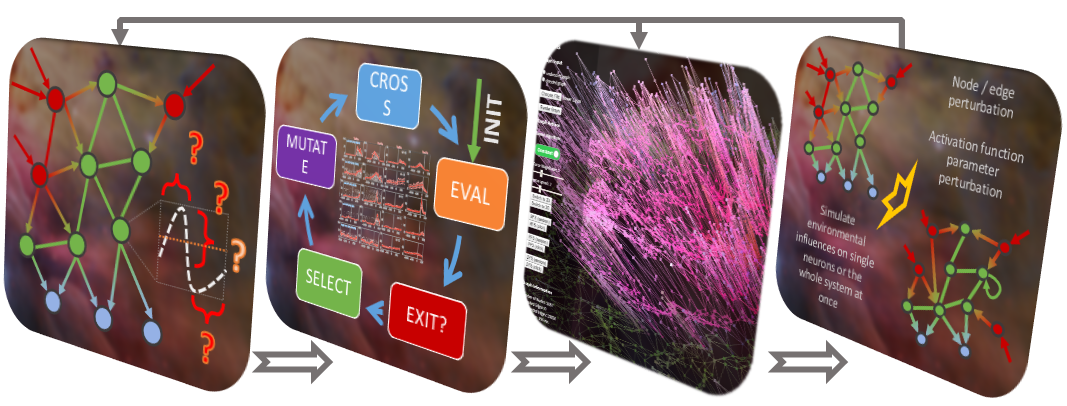
\includegraphics[width=\textwidth]{images/Pipeline}
\end{figure}
%
Graz, February, 1, 2017
% This is the "intended submission date" - to make it clearly beyond April, 1 

\end{center}
\vspace{0.5\baselineskip}
\end{titlepage}
%
%{\bf Project Team:} Andreas HOLZINGER (Lead), N.N. Postdoc, N.N. PhD - only when known in advance
% 1 PhD = 36,660 per year, or 109,800 for 3 years
{\bf Requested Funding:} 3 PhDs for the duration of 36 months
%\footnote{Note that this type of project is limited to a max. duration of 42 months}
\\[0,3cm]
%
%{\bf International Scientific Collaborators:} \\
%N.N. (US), N.N. (JP), N.N. (CA) - only if needed - think at first carefully at the reviewers
%
%here comes the OESTAT discipline from http://www.statistik.at/KDBWeb/kdb_Erlaeuterungen.do?KDBtoken=null&&elementID=7167147
%Computer simulation = 007, Data Mining = 033, HCI = 013, Informationdesign = 014, Machine learning = 019, Medical Informatics = 020, 015 = Information systems, 027= Web Engineering
{\bf OEFOS 2012 Discipline:} 102 Computer Science - 015  Information Systems 
\\[0,2cm]
%here comes the keywords, which are also important for reviewer selection, but please keep always in mind that the reviewers are selected from the related work: a) reviewers must be accessible (young enough, have time, not too famous),       b) no conflict of interest - no past joint work etc.
{\bf Keywords:} evolutionary algorithms, neuron simulation, connectome simulation, graph resilience, graph perturbation %connectome visualization, OpenWorm, connectome DSL, connectomes, c. elegans % NOTE: less keywords are better 
\\[0,2cm]
{\bf Note:} This proposal is original and has not been submitted to any other grant authority.
\\[0,2cm]
{\bf Ethical Declaration:} This proposal does not raise any ethical issues.
\\[0,2cm]
{\bf Remark:} This type of proposal is limited to a total number of 26 pages; as the duration of our PhD-program is 36 months this project has a duration of 36 months.
\newpage
%
%---page-02--- ensure appropriate page breaks
%
{\bf Abstract:}
\\[0,2cm]
% Make use of a graphical abstract as for example usual in ACM IUI
% \hl{NOTE: Emphasize that it is a hot and promising and raising topic and clearly outline what is the benefit of this project for the scientific community (be aware that the reviewer is part of THIS community!)}
% \hl{NOTE: It is essential to show the expected outcomes along the lines of methods, algorithms, tools, open source software, open data sets, publications in conferences and journals and organized workshops and conferences (as e.g. the HCI-KDD series!); Example: The contributions of this project to the international research community are in novel methods, algorithms, tools, a framework, Web-based ecosystem, and open data sets and publications in conferences and journals.}


This project aims to gain novel insights into standard connectome behavior and establish metrics of deviation from it, so we can effectively measure at which point the natural behavior of an organism collapses, which is a grand challenge and has many applications. As model organism we selected the c.elegans worm. A possible future noble prize would be to understand this worm - as most genes are shared with humans.
%At the very beginning it must be convincing what is the main question and why is this groundbreaking and will provide new results - the framework is a "by-product" of value of the others - always consider that the reviewer is part of the community: He must have a clear benefit if he grants this project.

As a big benefit for the international research community we will provide a framework for allowing non-programmers to conduct experiments on biological graphs in general and connectomes in particular. As the extent of this undertaking would be far outside the scope of any individual project with limited resources within a given time frame, we will focus on the example of the c.elegans connectome (which is already fully mapped and well understood) and provide a three-part pipeline as a basis for future extensions. In the first module we will investigate the degree of accuracy in connectome simulations sacrificed by the use of less biologically realistic neuron models, particularly in the context of simpler models usually requiring less cost in terms of processing power to run the simulation. To this end we will establish a baseline for the scientific community when deciding on the level of realism required for a particular study to yield feasible results while attempting to conserve processing power, especially with regard to simulating connectomes of more complex organisms in the future. In order to do this, we will implement a simulation framework tailored to our needs, which specifically means a high degree of modularity to support continually repeating the same study with several different neuron models. The second step will consist in making our findings available via a Web-based visualization framework, so that non IT experts like biologists or medical personnel can not only access but interact with our models. A vital part of this will be the introduction of a connectome-focused domain specific language (DSL) akin to well known database query and manipulation languages like SQL. This will also allow researchers to alter parameters of the underlying simulation on the level of individual elements (neurons, synapses, ion channels) as well as some system level (subgroups / the whole connectome) or even the environment. Based on the two modules above, the other great research goal is to test the resilience of already established neural networks with respect to perturbations, that is random (forced) reconfiguration of the internal connectome structure or environment influences on single components (disturbing forces on neurons and synapses). This project will employ 3 PhD students; since these students are expected to complete their degrees within three years, this effectively limits our time-frame to 36 months.


\newpage
%
%---page-03--- ensure appropriate page breaks
%
\vspace{\baselineskip}
\vspace*{10mm}
\tableofcontents
\newpage
%
%---page-04--- ensure appropriate page breaks
%
\section{Scientific Aspects}
\subsection{Motivation for our Research}
% \hl{NOTE: The reviewer has to answer the question AND to provide a grading 0-100 on "Importance to the international scientific community in the field X". A very short and concise summary WHY this research is necessary, interesting, and relevant - for the targeted scientific community; It should be made clear how the reviewers (as part of this community) may benefit from this project (open data sets! open source software! tools! etc.)}
%\begin{linenumbers}

The field of Connectomics is very promising in terms of furthering our understanding of nervous systems. While it has already very successfully increased our understanding of biological neural networks, connectomics still has several large challenges to overcome, to the point where over 20 years after the connectome of \emph{c.elegans} has been found as the first connectome of a multi-cellular organism, we are still not able to fully accurately simulate its nervous system, with progress for more complex neural networks lagging even further behind. There are several distinct obstacles that hamper progress within this field:
\begin{enumerate}
\item The data collection itself has several technical limitations imposed on it. In order to accurately not only map a nervous system anatomically in its entirety, but also find the appropriate parameters that govern the operation of every single cell and synapse within it, a large variety of different techniques need to be utilized, and some of those may prove impossible to perform on a given organism. For example the electro-physical properties of individual neurons of \emph{c. elegans}, which were impossible to measure due to the small size of the organism, were substituted by measurable values from the much larger \emph{ascaris suum} \citep{ThatBlueBook}.
\item As connectomics aims to analyze ever more complex organism, these technical difficulties get exacerbated by ethical considerations, which severely limit the possible techniques that can be employed.
\item Finally, all these problems get severely inflated by the sheer amount of data required.
\end{enumerate}

The combination of these issues means that finding the full connectome of any organism is a very lengthy task, albeit one that produces partial results at a constant rate. 

Some techniques have in the past been used to work around this problem. From a neuro-physiological point of view, some measurements that could not be conducted on e.g. \emph{c. elegans} have been conducted on closely related species, with the results being extrapolated \citep{ThatBlueBook}. More recently, evolutionary algorithms have been used to find missing parameters in order to be able to simulate the connectome accurately. This however introduces some parameters which are not (or at least, not yet) verifyably matching the actual neuro-physiological makeup of the original simulation target organism, raising concerns about how applicable the simulation is to this organism, or whether it is simply playing the \emph{imitation game}, approximating the desired behavior while maintaining completely different internal functionality.

So far complete datasets on complex organism, while certainly theoretically feasible, appear not achievable within the immediate future \citep{Gjorgjieva2014} \citep{Mikula2016}.


\subsection{Scientific Questions, Hypotheses and Goals}
% \hl{NOTE: The reviewer has to answer the question AND to provide a grading 0-100 on "CLARITY OF THE GOALS, HYPOTHESES"}

The main scientific questions in our project are aimed at \emph{feasibility} and \emph{scientific value} of the use of abstracted simulations in \emph {connectomics} as well as the examination of connectome resilience w.r.t. graph-theoretical measures. Having extensive experience in graph-based simulations and evolutionary algorithms we will evaluate the current state of such simulations and their applicability to future studies on more complex organism than \emph{c. elegans}.
%\\[0,2cm]

It is therefore our goal to explore and justify the following statements in detail. They are the key hypotheses of our proposal, and will be explored through the simulation of a specific connectome, namely that of \emph{c. elegans}:
\begin{enumerate}
\item Studies will be performed to prove that it is feasible to work with simulations of partial or simplified connectome models to obtain useful, if preliminary data. Considering the considerable time-frame involved in finding complex connectomes, this could lead to earlier preliminary insights into behavior by being able to simulate unfinished connectomes with a relevant degree of accuracy. It will also increase researchers' awareness of the exact degree of uncertainty inherent in the use of simplified models in this specific use case.
\item Considering the computational requirements for simulating the entire connectome, let alone running this simulation through an evolutionary algorithm, and the overarching goal of getting preliminary data from incomplete connectomes, it will be explored how far the computational model can be abstracted without influencing the results beyond tolerances.
\item As macro-scale connectomes have been used to gain valuable insights into the inner workings of human brains despite only providing a quite abstracted and simplified model, we will show that the same principle can be applied to micro-scale connectomes: Even simplified and incomplete models and simulations based on these can yield valuable insights and should be considered regardless of known or unknown deviations from biological realism in the details of neuron operation.
\item Since the current connectome for c. elegans is not entirely complete out of necessity, lacking some essential parameters for simulating exact neuron functions, the implementation will find these missing parameters by means of evolutionary algorithms, matching the evolved behavior as well as possible to the expected behavior as expressed by \emph{c. elegans}. The project will explore how much of the function of the connectome is predetermined by the physiological structure of it, and how much is governed by the exact parameters of the neurons - parameters which at least to a certain degree have the potential to adapt over time.
\item Pursuant to this the evolution will be repeated using different target behavior, in order to find the threshold at which the network as given is no longer able to perform the function due to it's deviation from the one the structure was intended for. In order to compare our model with the \emph{in vivo} behavior of \emph{c. elegans}, which we are not equipped to observe, we will be using the behavioral database published in \citep{yemini2013database}.
\item Our simulations can also be used to gain insight into the stability and resilience of the \emph{c. elegans} nervous system, which will give useful data as to how optimized biologically evolved networks actually are. This will be particularly useful in comparison to the extensive studies performed \emph{in vivo}, where single neurons were killed using a laser to understand the functions of those neurons and the effect of their death on the function of the neural network as a whole \citep{rothman2012caenorhabditis}.
\item Rounding off our project, we will show that a modern Web-based visualization and interaction framework using a simple, connectome-focused DSL can provide researchers outside the fields of IT and software engineering sufficient degrees of freedom to conduct professional experiments as the basis for future research, even on connectomes of more complex organisms.
\end{enumerate}


\subsection{Scientific Relevance and Innovative Aspects}
%\hl{NOTE: The reviewer has to answer the question AND to provide a grading 0-100 on "EXTENT TO WHICH THIS PROJECT COULD BREAK NEW GROUND SCIENTIFICALLY"}
Connectomics is a promising field of study to further our understanding of nervous systems. However, progress in this field is slow due to the sheer amount of data required and the difficulty in measuring that data. This problem has been worked around by using macro-scale connectomes, which do appear to provide useful data while still presenting a significant level of abstraction from the actual workings of the brain \citep{TheMissingArticle}.

Conversely, the field of micro-scale connectomics has focused on providing detailed data on the exact workings of neurons and their interconnections into a nervous system to the point of best possible match to known parameters from in vivo measurements. While this discipline focuses on accuracy, the amount of data to be measured is quite staggering. Also, as the example of \emph{c. elegans} shows, when the expected data set is completed, it often leads to important distinctions in hitherto disregarded details that need to be captured. For example, after simulations of \emph{c. elegans'} connectome failed to reproduce certain behavior, the role of neurotransmitters in shaping the functionality of the brain was re-examined and subsequently found to be necessary for biologically realistic simulations (\citep{Bargmann2012}, \citep{Izquierdo2013} and \citep{Ogg1997}).

Given this reliance on a set of data that can take enormous amounts of time to compile, the ability to work with incomplete datasets would allow further research, basing their studies on such simulations, to get a head start, thus allowing researchers to get preliminary findings before the dataset is entirely completed.

Another aspect of the same problem is the fact that accurate micro-scale simulations require vast quantities of processing power to complete. While this has proven completely necessary to accurately model the exact details of observed behavior, such simulations have existed before our understanding of neurophysiology reached its current level, and before computer equipment was as powerful as it is today. Even these earlier studies such as \citep{Kimura2005} were already quite successful in generating useful knowledge. This is an effect this project would like to investigate, as it proves that new insights do not necessarily require the best possible realism. 


\subsection{Importance of the expected results}
%\hl{NOTE: The reviewer has to answer the question AND to provide a grading 0-100 on "IMPORTANCE OF EXPECTED RESULTS FOR THE DISCIPLINE"}

The main areas of contribution will correspond with our key hypotheses as well as the work package structure that follows; therefore we content ourselves with a very concise list at this point:
\begin{itemize} 
  \item An evaluation of current and past simulation models for neuron function and neural network function in regards to their accuracy and processing simplicity. While research in this area tends to focus on finding the best possible accuracy, our evaluation will look at the trade-off between accuracy and processing power, and how much processing power can be saved by using a simplified model while staying within a given tolerance for the accuracy of the results.
  \item An evaluation of current connectome simulations concerning the divergence of results with different levels of abstraction and simplification in the details of the simulation will give valuable insight into how simplified data as a foundation for simulation can yield valuable preliminary results.
  \item Based on this evaluation a tool will be developed with the aim of providing researchers an accessible tool to simulate neural networks without specialist knowledge about the computer science behind it being required.
  \item In order to enable a fine-grained level of control not achievable by traditional user interfaces, we will define and implement a domain specific language (DSL) targeted specifically at interacting with the connectome of \emph{c. elegans}, but flexible enough to be extended to other organisms or biological networks in general.
  \item This tool will be used to conduct a study concerning the stability of the neural network of \emph{c. elegans}. Various detrimental stimuli will be applied to the network to gain data about which level of interference is required for certain functions to cease.
\end{itemize}


% \hl{NOTE: Discipline = Keyword = is defined via related work (Note: Authors of related work are potential review candidates IF they are still living, accessible and not stressed out!)}


\section{Work Plan}

The main workload involved in this project will be handled by three PhD students
supervised by the principal researcher and the international partners and supported by regular staff from the research group.
While the maximum time-frame for a project could be longer, we expect the PhD students to finish their degrees within three years. Thus, the overall duration for this project will also be limited to 36 months.

Our research will be split into 3 distinct work packages (WP), where WP 1 deals with evaluation of the current state-of-the-art for neuron and connectome simulations, as well as implementing our simulation framework based on these findings. WP 2 deals with visualization and editing of connectomes for use in our simulation engine, and WP 3 finally uses our completed framework to conduct stability studies on the connectome of \emph{c. elegans}.


% WP1 --------------------------------------------------------
\subsection{WP 1: Implementing the Simulation}

\textbf{Motivation:}
Most simulation tools that already exist in the area of connectomics attempt to replicate every known detail of the neural network, not just as a whole but also on a cellular level. While this has obvious accuracy benefits when attempting to discern the actual operation of neurons and their interconnectivity, it also bears a cost in terms of processing power requirements. If one is interested in investigating a more complex connectome than that of \emph{c. elegans}, one quickly finds the necessary computations exceeding the feasibility threshold.

Since this study attempts to research the applicability of simulations that use slightly abstracted neuron models in an effort to reduce this computational complexity, it will be necessary to implement our own simulations. As considerable effort can be invested in doing so, we will look at existing tools as a starting point, and aiming to adapt one of these as opposed to starting our own development from scratch. With this in mind, \emph{OpenWorm} \citep{Szigeti2014} appears to be a very promising tool for us to investigate, due to its modular design and multi-scale nature.

\emph{OpenWorm} is a simulation engine specifically tailored to \emph{c. elegans}, with the stated goal of the OpenWorm Foundation of providing simple access to in-depth simulation of the worm not only to researchers, but also to other interested parties such as artists or, in fact, any other interested individual. As such, it attempts to provide the greatest amount of accuracy in simulation while still providing a certain level of ease-of-use. In order to achieve this goal, an \emph{open science} \citep{nielsen2012reinventing} approach has been chosen for the project, with a large number of contributors still advancing the simulation. Since development on \emph{OpenWorm} began, parts of its core modules have already been updated to reflect new neuro-physiological findings about \emph{c. elegans}, increasing the complexity of the program while at the same time increasing its accuracy \citep{M.2013}.

Due to the open-science approach used by \emph{OpenWorm} and the resulting ease of access to the assets involved, as well as the modular nature of the implementation allowing for modification without prohibitive effort, \emph{OpenWorm} is likely a very suitable candidate for a starting framework which we can adapt to suit our needs.

However, due to the complexity of the software involved, this decision is not a trivial one, and some work must still be invested in evaluating the exact advantages and disadvantages of using \emph{OpenWorm} as a foundation for our work, as well as contrasting these with the benefits of other frameworks.
\\[0,2cm]

\textbf{Selected Related Work:}
As we are trying to implement not just a single simulation, but rather a modular framework able to cope with a variety of different neuron models, \emph{OpenWorm} is the natural prime candidate. The original rationale for the necessity for such a framework is presented in \citep{Szigeti2014}, whose authors also identify several of the key issues with integrative simulations in the field of connectomics, mainly in the use of traditional academic structures, which impede large-scale cooperation and sharing of data, which they overcome by using an open science approach. This gives us the advantage of not only providing the framework to build on, but also providing a platform for publicizing our findings after our studies are concluded.

The framework \emph{OpenWorm} provides has also in the meantime been expanded to include more and newer models to work with (for example \citep{M.2013}), proving that the goal of the original creators to implement a truly modular tool-kit was indeed successfully met.

The authors also explicitly state that the possibility of using different neuron models to investigate the relation between biological accuracy and the scope of behaviours reproduced by the simulation is indeed a secondary ambition of providing this framework ("As stated in the Introduction a secondary ambition of the project is to explore heuristically how the complexity of behaviors reproduced by the models scales with biological realism."  \citet{Szigeti2014}). However, to the best of our knowledge, such a study has not yet been conducted.

Other tools to be evaluated are the \emph{NEURON} simulation program \citep{Hines1994}, which, while providing good simulations of single cells and theoretically being able to simulate networks as well, includes no syntax for neural networks, and \emph{GENESIS} \citep{Bower2003}, which is commonly used by researchers when simulating large-scale neural networks. 

Finally, in order to support its effort to establish a standard format for connectome information, we consider it important to use \emph{NeuroML} \citep{Gleeson2010} for our simulation. This format is also already used by \emph{OpenWorm}, but even if we decide against that framework, \emph{neuroML} will be used by this project.
\\[0,2cm]


\textbf{Objectives:}

\textbf{O1: Definition of simulation requirements.}
As a first step in implementing our simulation or even evaluating existing tools the requirements for our studies need to be defined in order to provide a goal for the evaluation and subsequent adaptation. This in itself is no trivial task. While we attempt to study the effects of simplification and abstraction on the accuracy of these models, the exact nature of these abstractions must be chosen out of a very large selection of possible models, each having their respective benefits and drawbacks. 
%\todo{short example of different models (abstraction)}
Overall, since the aim is research into the effects of simplification on a model, several models with varying degrees of simplification from the state-of-the-art best fit to neuro-physiological data need to be evaluated in regards to their relevance and expected results.

%We consider it important though that the models chosen for this approach be chosen at this very early stage of the process, allowing the implementation to be tailored to their requirements. This mainly means a large amount of modularity and customizability in the finished simulation tools, in order to permit a large selection of models to be used in our study. However, since modularity and customizability in software usually comes at the cost of an elevated level of effort spent on the actual implementation, there is a certain trade-off involved, where some degree of flexibility of the framework may need to be sacrificed in order to allow for more time for the actual study. For this reason we must decide at the very least on a few types of models to use, as well as specifying their requirements on the simulation. This will be used as a starting point for the requirement specifications used for the next two objectives.


\textbf{O2: Evaluation of existing tools.}
Instead of implementing an entire new simulation framework, our focus will be on the adaptation of an existing one, probably \emph{OpenWorm}. This framework is very modular, a fact that has been used in the past to update its internal workings to accommodate newly discovered neuro-physiological insights. However, simplifying this tool from its original form has not yet been done to the best of our knowledge. Also, the tool's development has been focused on the connectome of \emph{c. elegans}, with the possibility of also simulating other neural networks so far not explicitly featuring in any documentation. However, it is still possible that \emph{OpenWorm} does include such a possibility with only minor adaptation. While \emph{OpenWorm} seems to have the most potential as a base for our implementation, we will also evaluate the \emph{NEURON} and \emph{GENESIS} simulations. These do not provide an entirely integrated simulation framework, but offer the basic simulations we could build our toolset around. Even if \emph{OpenWorm} proves to be the best candidate, these other tools will still be evaluated in order to gain an overview over the current landscape of neuron simulation tools.

\textbf{O3: Creation of a simulation toolset}
After deciding on which framework to use and how it must be adapted, the next step is to actually implement the simulation according to our specification. This not only means adapting parts of the selected framework to our purpose (such as replacing the neuron model), but also implementing several alternative models (such as one for neurons affected by a disease) that will subsequently be used in our simulations to emulate faults in the system.

\textbf{O4: Design of an Evolutionary Algorithm.}
Finally, based on the adapted simulation, an evolutionary algorithm will be construed in order to not only find, but also fine-tune the various parameters within the connectome. While this has been done on \emph{c. elegans} and the resulting datasets are available (amongst others as a part of the \emph{OpenWorm} framework as detailed in \citep{Szigeti2014}), part of our study will necessitate some new fine-tuning, in order to adapt the network to a slightly abstracted operation of the single neurons that compose it.
\\[0,2cm]

% This also means that this evolutionary algorithm should be flexible enough to deal with bigger and more complex connectomes in the future, in order to provide a tool that is not only useful for \emph{c. elegans}, but has a large variety of possible applications in future connectomics research. This will explicitly have to include an implementation that deals with the technical problems of simulating and evolving a large connectome, such as the immense amounts of data needing to be handled, even though this is not a problem we will encounter as part of this project directly.


\textbf{Tasks:}

\textbf{T1: Identification and specification of suitable neuron and neural network models for use in the study.}
While this point could be designated as a simple starting point for the remainder of this project, we are committed to providing a thorough analysis on the advantages and disadvantages of each possible model, to the point where the output should be in-depth enough to qualify for publication as a paper on its own merit without relying on the remaining parts of this project for substance.

\textbf{T2: Evaluation of existing tools.}
We will evaluate \emph{OpenWorm}, as well as several competing simulation tools, particularly their inner workings for compatibility with our goals.

\textbf{T3: Adaptation of chosen tool and implementation of additional features.}
Even adapting an existing tool for our purpose, there will be some features we will have to implement ourselves. The main goal is to have the simulation as adaptable as possible in order to deal with a lot of potential scenarios during the actual studies.

\textbf{T4: Implementing the Evolutionary Algorithm.} While this can be based on preexisting work, some implementation effort needs to be expended for adaptations. Furthermore, our tools are meant to be usable with other connectomes in the future. These connectomes may not be as complete as our current understanding of \emph{c. elegans}, and may therefore require this algorithm to find missing parameters before a simulation can be conducted. Finally, the algorithm needs to be able to cope with potentially much larger datasets.
\\[0,2cm]



\textbf{Deliverables:}

\textbf{D1: Connectome of \emph{c.elegans}.}
The complete c. elegans connectome with the parameters found by the evolutionary algorithm will be published, to allow for easy verification of the results. As matching the found parameters with the actual physiological properties of the neurons would certainly be beyond the scope of this project, it would benefit future research if this data were to be compared by a more neuro-biologically minded research group to comment on differences or similarities.

One comparison however is possible: The comparison between our dataset and ones previously discovered by evolutionary algorithms, where possible by algorithms using the simulation chosen as the base for our study. This will allow us to find similarities and differences, highlighting the impact the altered simulation model has on the final result. Some results, such as some information paths being vastly different as a result of minor differences in simulation accuracy, will yield new insights into the way neurons interact and how stable and/or adaptable a biological neural network is. This comparison will be submitted for a conference, e.g. NIPS. 

%\todo{The conferences which we really want to target, e.g. NIPS, but for this we have to reference at least one - to show that this might fit in}


\textbf{D2: Specification of suitable models and their benefits / drawbacks when used in a simulation, along with their requirements for the simulation.} This deliverable is considered to be substantial enough to warrant publication as a paper in a journal such as Springer KAIS or Springer BRAIN.

%\todo{@Andreas: journal or conf?}

\textbf{D3: Simulation framework.} The base simulation framework along with the implementation of the evolutionary algorithm will be published as open-source software hosted on GitHub. As one of the main tasks of this project, the work should provide sufficient material to support a paper regarding the implementation well before completion. Furthermore, the completion of this task should also be presented at a suitable conference and/or workshop in order to inform the scientific community at large of our ongoing efforts.
\\[0,2cm]



% WP2 --------------------------------------------------------
\subsection{WP 2: Visualization and Connectome Editor}

\textbf{Motivation:}
Once the simulation is operational, it will be important for researchers to be able to use it effectively, preferably without the need for specialist knowledge in the exact function of the simulation itself. Even if such knowledge is present, it is a large time investment to have to interfere with the simulation's code every time a minor adjustment needs to be made. While this is generally true, it holds particular relevance here, since our study will revolve around conducting a similar experiment in the simulation repeatedly, adjusting parameters and neuron models between runs. As simulating the connectome is a rather computation-extensive process, the resulting patterns can be very complex and difficult to read from tables of numbers alone. It is therefore necessary to implement a visualization tool that allows researchers to \emph{see} the connectome in operation, in order to benefit from humans' ability to detect patterns and changes in them visually.

Our project team has experience in graph visualization from the creation of \emph{Graphinius}, a tool consisting of an underlying graph library as well as a visualization module hitherto used to display 3D graphs extracted from medical images \citep{GraphExtractPaper}. On this basis our goal is to create a front-end for our simulation, which will not only provide an accessible way of defining the parameters of a simulation, but also serves as an easy way to observe the function of the connectome in a real-time and interactive manner.


Once the simulation has been established, our next step is to provide researchers an easy way to manipulate the connectome and / or environment parameters. Whereas easy functions such as ambient temperature might be accessible via simple UI elements, more complex interaction scenarios call for fine grained control: Imagine e.g. a researcher wanting to modify the steepness of interneurons' activation functions in dependence of it's neighbors and / or importance in the connectome - this would be hard to implement via a UI element, but it's easy to imagine being done via a SQL-like query (\textit{"SELECT INTERNEURONS where DEGREE $>$ 5 SET ACTIVATION STEEPNESS TO 15;"}).

Such a \textit{domain specific language (DSL)} can be defined as the 'ultimate abstraction' of a problem domain \citep{Hudak1998DSL}, insofar as it is Turing complete within its domain (every conceivable problem inside the respective domain can be expressed by it) but not Turing complete in a general sense. To a non-programmer it provides an intuitive abstraction of the inner workings of a given domain, offering constructs to access its elements on different levels of abstraction as well as expression functional statements (rules) concerning those elements. In the context of our connectome simulations, the set of elements will most likely consist of different types of neurons and synapses, but could also comprise smaller elements like ion channels or larger ones like connectome components or the whole connectome itself.

According to \citep{Deursen2000DSLImplementation} there are several ways to implement a DSL: 1) Interpretation or compilation from scratch, which has the advantage to be unrestricted in its usage of constructs, but the disadvantage of being the most expensive approach. 2) Using an embedded language, where base constructs of the host language are re-used to build higher-abstracted features; this raises the problem of limited expressiveness. 3) Preprocessing or macro-processing, where pre-defined string sequences are translated into host language constructs; this results in a simple processing chain but unoptimized, brittle code constructs; and finally 4) using an extensible compiler or interpreter combining preprocessing of macros with a compiler / interpreter capable of doing (AST) optimization or static checking. For our project we are going to take a look at the implementation of \emph{SQL} as well as \emph{Cypher}, \emph{Neo4j}’s query language, the latter of which was already designed to operate on graph structures.
\\[0,2cm]


\textbf{Selected Related Work:}
While the exact requirements on the editing part of this work package will be defined as part of \emph{WPs 1 \& 3}, the visualization part will be more interesting from a technical point of view. As mentioned before we will base this tool on our already emerging \emph{Graphinius} framework which at the time of this writing is capable of handling graphs of up to 130k nodes and 300k edges - this far surpasses the capacity of other Web-based graph visualization libraries which often max out at graph sizes two orders of magnitude below (and we are far from finished optimizing it...). Regardless of this we will also evaluate other existing tools for features potentially relevant to our effort. Specifically we will look at the \emph{neuroConstruct} and \emph{ConnectomeViewerFramework}.

%\emph{NeuroConstruct} \citep{Gleeson2007} as a tool is an inspiration of what we want our editing tool to be. It allows for the definition of cell models, the free construction of a neural network based on these single cells in 3D space, and the automatic generation of script files for simulator packages to carry out simulations. It does however only support NEURON \citep{Hines1994} and GENESIS \citep{Bower2003} as its simulation engines. It also allows the finished simulation to be loaded for visualization, which is certainly a desirable feature for researchers and supports NeuroML. On the other hand the newest available version of this library is from 2012 indicating that further development has been abandoned.

%\emph{ConnectomeViewerFramework} \citep{Gerhard2011} on the other hand does not support NeuroML, and while the user interface promises a higher degree of usability than \emph{neuroConstruct}, it also requires the user to have some knowledge of Python and requires a local installation. However, it does have superior support for large-scale connectomes and their visualization. Since one goal of this project is compatibility with more complex connectomes, some of the best practices of large-scale connectome visualization need to be taken into consideration, as displaying such vast quantities of individual neurons would no longer be human-readable.

As far as existing DSL implementations for biological networks are concerned, two projects have stirred our interest: \emph{Eugene} \citep{Bilitchenko2011Eugene} follows the approach of \textit{synthetic biology}, which means the application of engineering principles in biological domains. It supports as its elements 1) Parts, which represent basic biological entities (e.g. DNA sequences, Promoters, Terminators), 2) Devices representing composition of parts encoding a certain functionality, and 3) Rules for how those elements may interact. The goal of \emph{Eugene} are design space exploration, simulation as well as automated assembly.

The \emph{GReg} (Gene Regulatory) project \citep{Sedlmajer2012Greg} arose from the insight that cellular and supra-cellular interactions are hard to investigate because of exponential explosion; (IT) model checking approaches on the other hand are already able to deal with such problems (symbolic encoding of the state space, for instance). The \emph{GReg} represents a simple DNA-to-protein processing chain by encoding relevant portions of DNA (Initiation, Operation, Termination, Non-Termination) as well as cell network components (Organelle, Cell, Network). It further consists of the \emph{GReg} language / component specification for molecules, reactions, chromosomes, genes and a \emph{GReg} query language (GQL) to capture component interaction.
\\[0,2cm]


\textbf{Objectives:}

\textbf{O1: A Connectome Visualization} based on \emph{Graphinius} capable of presenting the structural layout of the connectome being simulated as well as the current state of the network. There are also two time-scales necessary for this tool to operate on: given our goal of providing tools that will be able to deal with more complex connectomes in the future, we must assume that the complexity of the network being investigated may be more than we are able to process in real-time, necessitating the visualization to run as slow as the simulation. On the other hand, the simulation will produce output which can be viewed at a later date, at which point the visualization should be able to run in real-time.

\textbf{O2: A Connectome Editor} based on a DSL so that the network to be simulated can be easily manipulated by researchers without expert knowledge in programming. This editor will allow not only the alteration of parameters within the existing connectome structure, but also the adding and removing of neurons and synapses (graph perturbation), as well as the editing of parameters of the simulation itself. Importantly, it will also permit the swapping of the used neuron models for individual neurons, which will permit the simulation to emulate certain conditions where single neurons suffer from some restriction of their function, such as MS \citep{Hauser2006}. It will also seamlessly integrate with the evolutionary algorithm in order to fine-tune the network to the changed parameters.
\\[0,2cm]

%\textbf{O3: Expanded Control through the Visualization}
%With the editor and its methods of altering the base connectome data in place, the visualization tool will be expanded to allow limited control over the network during operation. The expected use case for this would be stability studies, where the connectome is running within parameters as usual when some part of its operation is compromised, as can happen in nature through injury or illness.

%\textbf{O4: Ease of Use}
%This study, and the toolset it provides, will require a certain amount of effort for setting up for each individual study performed. It is thus our goal to also implement tools that allow this process to be performed through an easy-to-use editor that would not only cut down on the time required for this initialization, but also allow researchers without expertise in programming to use our tools effectively. \todo{@Bernd: put into WP2}


\textbf{Tasks:}

\textbf{T1: Extending Graphinius} to work specifically with connectome graph structures and interact seamlessly with the core simulator including its evolutionary algorithm. Also create a User Interface for simple navigation / interaction with the underlying network.

\textbf{T2: Connectome Alteration Language.} Design a DSL as described above, probably based on the \emph{GReg} framework but taking connectome-specific elements and interactions into accound. This standardized language will also permit graph perturbation and thereby greatly improve the range of experiments which can be conducted.
\\[0,2cm]


\textbf{Deliverables:}

\textbf{D1: Connectome Editor.} The output of this module will primarily be a set of open source software libraries published on GitHub as well as a technical paper describing its development process and intricacies, to be published e.g. in \textit{IEEE Software}.
Note: if we propose to 

\textbf{D2: Connectome Alteration Language.} The output of this module will primarily be a DSL specification along with an open source software implementation; a demonstration paper will be published, e.g. in \textit{IEEE Signal Processing Magazine}.



% WP3 --------------------------------------------------------
\subsection{WP 3: Conducting graph resilience studies}

\textbf{Motivation:}
With both the simulation and the visualization / editing module in place, we can now perform studies to explore the level of distortion we can apply to the connectome before either some predetermined network metric disappears (diverges beyond a set threshold) or some predefined behavior collapses in the simulation. As a first step, by repeating some connectome stability studies performed \emph{in vivo}, such as \citep{Avery1989473}, we will obtain examples which we can further on use as a ground truth, giving us information about the accuracy of our simulation. This cannot just inform us about the natural flexibility of the \emph{c.elegans} connectome but will ultimately be used to generalize about the effectiveness of utilizing simplified models (on all levels of the underlying graph structure) to gain preliminary estimates about the accuracy of more complex connectome simulations in the future (for instance w.r.t. missing data). But first let's pause to consider what graph resilience even means and where it finds natural applications inside and outside the biological domain:

According to \citep{Sudakov2008LocalGlobal} the resilience of a graph $G$ with respect to a property $P$ measures how much one has to change $G$ in order to destroy (invalidate) $P$. They further distinguish between \textit{global} and \textit{local} resilience, where the former measures how many perturbations on a graph level (individual distortions) one has to inflict before the property $P$ breaks down, whereas the latter indicates how many perturbations on a local level (on each vertex) a property $P$ can endure. This leads to the somewhat counter-intuitive notion that if the property $P$ is local, it makes more sense to talk about global resilience, whereas if the property $P$ is global, the local resilience is the more meaningful measure.

An interesting issue is the inherent perturbation of biological models mentioned by \citep{Hendrix2010MaxCliqueTheory}, who states that in many biological systems the underlying (sensory) data are so noisy that graph models can only be constructed by assigning a likelihood threshold above which an edge is said to exist in the graph. Different settings of this threshold would therefore result in differently perturbed models of the underlying, inaccessible information. Even before this publication, \citep{Samatova2008GraphPerturbationScalableAlgorithms} have already introduced their "Graph Perturbation Theory" which states that if a solution to a reference graph is known, exact solutions for graph measures of perturbed graphs can be found by computing the difference set; they proved their theory on the Maximal Clique enumeration problem using efficient indexing which lead to an 80\% decrease in computational cost compared to traditional methods. Although this insight is not vital for our project starting with \emph{c.elegans}, it might prove useful when expanding to more complex connectomes.
\\[0,2cm]


\textbf{Selected Related Work:} Lets now take a brief look at the significance of graph resilience / perturbation in different fields of applications; although they may not seem directly relevant to our simulations, they could sill provide fundamental ideas or insights that will help us over the course of this project:

In computer networks, massively parallel processing systems rely on node connectivity and the failure of a node can not only disrupt, but also affect rollback and recovery of a transaction. In an early work, \citep{Gaudiot1990NetworkResilience} already introduced resilience under the name of \emph{fault tolerance} and differentiates between dynamic system which can reconfigure their topology in reaction to node failures, and static systems which can not. They define \emph{k-fault tolerance} as the ability of a system to withstand the failure of up to k nodes. The weakness of their work is it's assumption of regular network topology which - to our best knowledge - cannot be guaranteed in biological networks.

In transportation networks, resilience can be understood as the ability of a system to return to a stable state following a strong perturbation caused by failure \citep{Ip2011ResilienceTransportationNetworks}; its influence factors are described as 1) redundancy of resources, 2) distribution of supplies and 3) reliability of delivery lines, all three of which would find easy pendants in connectomes. The authors also introduce the term \emph{friability} which measures the reduction of total resilience upon removal of a particular node or edge (and thus measure the importance of it).

In complex networks, the overall resilience depends strongly on the underlying topology, as  \citep{Ash2007CascadingFailures} argue; they specifically discuss scale-free (power-law distributed) graphs and contrast their robustness against random node failures with their susceptibility to losing important hubs. Even more so, when hubs are 'removed', such networks can disintegrate rapidly. Therefore, the authors conducted experiments in which they grew networks employing an evolutionary algorithm and observed different topologies behave under perturbation. Their results show that graph metrics like typical path lengths, clustering (e.g. small-world phenomenon) and modularity play an important part in the design of robust large-scale infrastructures.

As \citep{Sauer2004CellularFunction} state, biological systems maintain phenotypic stability in the face of diverse perturbations arising from environmental changes, stochastic events, intracellular noise and genetic variation. However there is still no common agreement on what robustness precisely is and how it is accomplished at the cellular or molecular level. As graph measures are concerned, there is a difference between assortative mixing in biological vs. general networks \citep{Piraveenan2012AssortativeMixing}, insofar that most biological graphs are directed and therefore the traditional measure of assortativity has to be redefined; e.g. regulators with high out-degree have maximum influence if the nodes they regulate have high out-degree as well.

Arriving at the human brain, \citep{Peters2013BrainFunctionalNetworks} investigating altered connectivity in neurological disorders. They conjectured that some classes of disorders can actually be seen as disconnection syndrome within the brain's connectome and focused on Tuberous Sclerosis Complex (TSC - a genetic neurocutaneous disorder) and autism spectrum disorders (ASD). After EEG data were collected from different groups of patients, graph measures of the functional networks were computed and a resilience analysis was conducted. This revealed connectivity differences from healthy connectomes specific to TSC and ASD, and these differences were very consistent across subgroups. In TSC, both with and without a concurrent diagnosis of ASD, mean coherence,
global efficiency, and clustering coefficient were decreased and the average path length was increased. These findings indicate an altered network topology.
\\[0,2cm]


\textbf{Objectives:}

\textbf{O1: Connectome resilience data}. First, we need to find out which graph metrics are most vulnerable to perturbations of the \emph{c.elegans} connectome. One obvious question to ask here is whether to only go for singular metrics or also inspect possible combinations and if the latter, what sets of combinations. We can then gain insights into what perturbation methods have the least / greatest effect on the network stability. Possible candidates are the classic perturbation via adding / deleting nodes or edges, but more sophisticated approaches like neuron activation function parameter distortion or even targeting specific graph metrics like modularity or path lengths might be in order. Once this knowledge is obtained, we will strive to come up with measures to counteract especially dangerous perturbations in order to stabilize a connectome. If we succeed on a fundamental, theoretical level, this alone might yield innumerable applications in health care.

\textbf{O2: Perturbing the connectome via accuracies of neuron models.} As in a section mentioned above, the inaccuracy of sensory data in biology can lead to graph perturbations that manifest in a different level of accuracy in the description of the (invisible) ground truth. We are therefore going to abstract the \emph{c.elegans} connectome in different ways to observe simulation behavior w.r.t. input granularity.


\textbf{Tasks:}

\textbf{T1: Running connectome resilience simulations.} 
We are going to start with a whole set of graph metrics and filter the combinations that seem to contribute most to the overall connectome stability. Then using our own framework, we will choose suitable perturbation methods to provoke a collapse (intolerable deviation) of those metrics. We will repeat those experiments with different combinations of target metrics and perturbation methods, creating a list of the deadliest (most benign) 'attacks' a \emph{c.elegans} can be exposed to. In phase 3, starting from already perturbed (non-functional) connectomes, we will introduce 'positive perturbations' to reverse the effects caused and heal the organism. The algorithms applied in step 3 will of course be oblivious to the methods used in step 2.


\textbf{T2: Studies on the simulation behavior w.r.t. model accuracy.}
The simulation chosen to test our hypothesis is a study concerning how damage to entities in the network (single components or wholes subgroups) affects the function of the network as a whole. Subsequently this study will be repeated using different simulation models with varying degrees of accuracy. The goal is to ascertain the extent to which the found results will differ given these varied models. This will show how much variations in accuracy of the used model actually influence the end results of the study, shedding light on the usefulness of simulations using simulations which may not be state-of-the-art in terms of simulation accuracy, but bring benefits in the use of processing power.
\\[0,2cm]


\textbf{Deliverables:} 

\textbf{D1: Connectome Stability data and survey.}
The algorithms and hyperparameters produced will be made available via an open-source license and hosted on GitHub to facilitate easier studies in the future. Moreover, a comprehensive survey of our findings will be published in a suitable journal, e.g. Springer BRAIN.

\textbf{D2: Analysis of the impact of different accuracies of neuron models on the results of connectome simulations.} This will be an in-depth analysis of the results of our overall project. We will present those findings at an international conference, e.g. Gecco, and expand it into a suitable journal.


\newpage

\section{Organizational Aspects}

\subsection{Work Organization, Supervision and Risk Management}

The lead applicant, Andreas Holzinger, will act as project leader and will work directly on this project and allocate a significant amount of time to the X-CORESIM project. He is associate professor for Computer Science and a member of the doctoral school for Computer Science at Graz University of Technology, hence he is in the position to supervise the involved PhD students and to bring in new or additional work-force on demand.

He has extensive project management experience and know-how in software development and his diverse scientific background will be a further success factor for this project. Moreover, this project has the full commitment of the Holzinger Group, the applicant's institute and the University, so all technical facilities and organizational support is ensured.

We take care on risks at three levels (scientific risks, management risks, technical risks):
\\[0,2cm]
\textbf{Scientific risks} lie in the uncertainty of research. We follow the approach that key elements in managing uncertainty are reflective learning and sense-making as well as a good communication strategy and a well-balanced atmosphere to stimulate thinking and problem solving. 
%\citep{Holzinger2010ProcessGuide}. 
We take measures to control progress of work, ensure detailed and clear definition of architecture/interfaces and focus on implementing key features in sane iterations. To further reduce risks we have incorporated an international Scientific Advisory Board and will ensure regular communication/feedback. 
\\[0,2cm]
\textbf{Managerial risks} include lack of resources and/or staff changes forced upon the project by one or more collaborators, therefore the quality of the outcome might decrease as it depends on having access to high-quality resources and staff. We will ensure a good level of communication to talk about any problems that arise and will strive to quickly bring in new scientific staff if necessary. For this we are well prepared as we can allocate additional human resources from permanent staffs at short notice.
\\[0,2cm]
\textbf{Technical risks} may include difficulties in data acquisition. This risk is minimal, since we are planning to use publicly available data sets throughout the project. All equipment is at our disposal and this project has full commitment by both our Institute and University.

\subsection{Strategies for Dissemination of Results}

\textbf{1. Science-to-Science:} We will produce internal progress reports. The most promising ones will be extended to peer-reviewed conferences papers, symposia and workshop contributions and the most valuable results will be developed into solid international journal publications. The project team also plans to organize workshops/special sessions at international conferences to disseminate the gained knowledge, and to make algorithms and tools accessible to the international scientific community. The lead applicant has established an HCI-KDD expert network since 2011, which will also serve as an international dissemination platform.

\textbf{2. Science-to-Business:} As our algorithmic libraries will be open source and available online, businesses might find it interesting to utilize or embed our software in their products, although we have no co-operation with existing commercial vendors of KDD software at present.

\textbf{3. Science-to-Public:} We will inform the public about our research and aim to disseminate our knowledge broadly on a regional level, for example in public exhibits, at public Open-lab days ("FWF Lange Nacht der Forschung" and "ARRS Night of researchers", in regional as well as international workshops, etc. A project web-site based will be available and provide a public showcase similar to WormSIM.

\subsection{Economic, Social and Practical Impact}
% \hl{NOTE: The reviewer has to answer two ADDITIONAL questions on 'Is the project expected to have implications that go beyond basic science - potential industrial applications, results of relevance to society etc.?' and 'CAN THE PROJECT BE EXPECTED TO HAVE IMPLICATIONS FOR OTHER BRANCHES OF SCIENCE'}


The main goals of this project are on facilitating future connectome studies by 1) giving researchers the tools to accelerate future connectome studies, by allowing simulations to save processing power where absolute accuracy is not required, 2) enabling simple, immediate visualization and interaction with results including the possibility to modify simulations without expert knowledge in computer science, and 3) giving researchers in the fields of biology / medicine the ability to define detailed connectome resilience studies out-of-the-box. While the ensuing knowledge gain is mainly of use for the research community, the tools we are going to develop in the process might lead to a general acceleration of neuro-physiological research and the understanding of the brain it promises; we believe this could have a significant impact on the future of medical developments.

An increased understanding of neuronal computations would also lend itself to a new generation of engineering applications. As an example, the motion detection circuit of \emph{Drosophila melanogaster} has been identified, which brings with it the potential to include these findings in motion detection solutions \citep{Takemura2013}.


\subsection{Career Benefits for those Involved}
% \hl{NOTE: The reviewer has to answer the question AND to provide a grading 0-100 on "EXPECTED IMPORTANCE OF THE PROJECT FOR THE CAREER DEVELOPMENT OF THE PARTICIPANTS (PROJECT LEADER AND CO-WORKERS)"}

The PhD students involved will have an excellent opportunity to achieve knowledge in an extremely interesting and stimulating setting within a realistic time horizon. There are several promising research directions worth being pursued as a PhD within this project. 

All project members have the opportunity to achieve expert know-how in an area that is becoming ever more important in the future, particularly considering full connectome simulations of complex organisms are already on the way.


\subsection{Infrastructure}

The project applicant is mainly employed at the Institute for Medical Informatics, Statistics and Documentation, Medical University Graz where he is heading the Holzinger Group HCI-KDD. Andreas and his Group work on a synergistic combination of methodologies of two areas that offer ideal conditions towards unraveling problems in data science: Human-Computer Interaction (HCI) and Knowledge Discovery/Data Mining (KDD), with the goal of supporting human intelligence with machine learning to discover novel, previously unknown insights into data. The group is embedded in the institute, which has long-standing experience in biomedical information systems, with emphasis on making clinical data usable. This includes the development and evaluation of algorithms, software and statistical methods, from data acquisition to data analytics. The Institute offers statistical expertise for biomedical research projects, data management for clinical trials and data extraction and reporting services for medical research. The dedication is to deliver high-quality, methodical contributions and to develop software systems for the support of clinical researchers with a focus on information quality. The Institute maintains a Quality Management System, has long-standing software engineering expertise, and is ISO 9001 (certification number: Q-11627/0) certified in both project management and software development. All necessary equipment is available and this project has the threefold support of the Holzinger-Group, the Institute and the University.



\subsection{National and International Cooperation}
% \hl{NOTE: The reviewer has to answer the question AND to provide a grading 0-100 on "Quality of the cooperations - both national and international"}

The lead applicant is employed at the Medical University Graz, located at Graz University Hospital, where excellent local co-operations to relevant biological domain experts are established. The applicant is Associated professor at Graz University of Technology, where he teaches the main required lecture Biomedical Informatics at the Faculty of Computer Science and Biomedical Engineering and supervises engineering students. Additionally, the project applicant is Visiting Professor for Machine Learning in Health Informatics at the Vienna University of Technology - therefore a cross-disciplinary knowledge exchange between health informatics and engineering is ensured. On an international level the group is well connected to the international HCI-KDD network, which the project applicant established. To guarantee that X-CORESIM will be successful, we will provide international workshops to exchange knowledge with international colleagues whose use cases connect to ours.

\subsection{Project Team}
Note: Short CVs of team members are attached in separate documents

\textbf{Assoc.Prof. Dr. Andreas HOLZINGER} is the project applicant and principal investigator, head of the Research Unit HCI-KDD at the Medical University Graz, and currently Visiting Professor for machine learning in health informatics at Vienna University of Technology. His interdisciplinary experience in management of national and European Projects will be very beneficial in this project. He will support and supervise the PhD students closely together with the internatioal experts.
\\[0,2cm]
\textbf{Prof. Dr. Matthias DEHMER} is the mathematical expert in our project and will particularly help in supervision of the PhD students and in dissemination of the results to the international research community. Matthias is currently Professor at Nankai University, Tianjin, China and he is an expert in graph theory, data science,
complex networks, complexity, statistics and information theory. He has published extensively in data science and structural network analysis.   
\\[0,2cm]
\textbf{Prof. Frank Emmert-Streib} is the computational biology expert in our project and he will help particularly in the supervision of the PhD students and in dissemination of the results to the international research community. His expertise includes computational biology, biostatistics, and machine learning in the development and application of statistical analysis methods to investigate high-dimensional data. He has worked on problems from neurobiology, molecular biology, web mining, chemistry, and physics. He is currently Professor at the Tampere University of Technology, Finland, focusing on the analysis of high-throughput data from complex diseases and digital business.  
\\[0,2cm]
\textbf{Bernd Malle, PhD student}
Bernd has finished his Master studies in Software Development at Graz University of Technology, supervised by Prof. Holzinger. He is interested in graph based Machine Learning and initiated the project 'Graphinius' connecting a graph library to an in-browser code editor \& visualization module. The combination of theoretical interests and practical ambition makes Bernd an ideal candidate for this project, with a particularly good match for the connectome resilience studies.
\\[0,2cm]
\textbf{Wolfgang Scherer, PhD student}
Wolfgang completed a MSc by Research in Electronics from the University of York (UK) with his thesis "Training Spiking Neural Networks by Evolutionary Algorithms." He is now finishing a second Master degree at Graz University of Technology in Software Development supervised by Prof. Holzinger, which he will have completed by the time this project commences. With his previous work on simulations of neural networks as well as evolutionary algorithms, he is a very good candidate for implementing the tools in question.
\\[0,2cm]
\textbf{1 x N.N. PhD} One more PhD student will be hired once the project has been granted and will be working mainly on the visualization platform as well as implementing appropriate DSLs for perturbation experiments in close cooperation with Bernd.
\\[0,2cm]
It should be noted that although the work packages have been split amongst the PhDs, this only refers to overall responsibility and supervisory aspects for these packages. The PhD students will be jointly working together on all work packages for the duration of the project.

% All personnel should be justified and explained what and with whom they are working


\section{Financial Aspects}
%
%\subsection{Total Project Costs}
% \hl{NOTE: The reviewer has to answer the question AND to provide a grading
% 0-100 on "APPROPRIATENESS OF THE FINANCIAL PLANNING"}
% NOTE: Make it as simple as possible - no complicated structure - just three PhDs - that's it - no Masters or Bachelors!

\subsection{Grant applications of partners}
In order to successfully carry out this project three full time PhDs over the whole project duration of 36 months is needed. 
%This results in 345,940 EUR, to which the obligatory overhead of 5\% must be added, which results in the total grant application of \textbf{363,237 EUR}.
\\[0,2cm]

\subsection{Funding per year}
\begin{table}[H]
   \begin{tabular}{| p{4.6cm} | >{\hfill}m{2cm} | >{\hfill}m{2cm} | >{\hfill}p{2cm} | >{\hfill}p{2cm}| }
   \hline
   \rowcolor{Gray}
   \textbf{} & \textbf{Year 1} & \textbf{Year 2} & \textbf{Year 3} & \textbf{Total} \\  \hline
  Bernd MALLE   & \EUR{36,660} & \EUR{36,660} & \EUR{36,660} & \EUR{109,980}  \\ \hline
    Wolfgang SCHERER   & \EUR{36,660} & \EUR{36,660} & \EUR{36,660} & \EUR{109,980}  \\ \hline
    PhD N.N.   & \EUR{36,660} & \EUR{36,660} & \EUR{36,660} & \EUR{109,980}  \\ \hline
    MSc N.N.   & \EUR{17,320} & \EUR{17,320} & \EUR{8,660} & \EUR{0}  \\ \hline
    \textbf{Total project costs} &  &  &  & \EUR{373,240}  \\ \hline
   5\% obligatory Overhead &  &  &  & \EUR{18,662}  \\ \hline
   \textbf{Requested funding}  &  &  &  &  \EUR{391,902}  \\
   \hline
   \end{tabular}
   \caption{Requested funding per year.}  
 \end{table}

For this project we have set up a team contributing to the project on an in-kind basis. These include the experts listed above, senior staff costs from the hosting institution, additional support staff, organization of international workshops, all necessary equipment, open access costs, and all travel costs will be covered by in-house budget or other specific travel grants. 



\vspace{1cm}

% \newpage
\bibliographystyle{apalike2}
%\makeatletter
%\renewcommand\@biblabel[1]{#1. }
%\makeatother

\setstretch{0.6}
%\def\bibfont{\footnotesize}
% \setlength\bibsep{0.8\baselineskip}
\section{References}
Note: Due to the page limit, this list contains only limited related work.
\begingroup
\renewcommand{\section}[2]{}%
\\[0.3cm]
\bibliography{Bibliography,graphDSLs,graph_perturbation_resilience}

\begin{center}
\vspace{1cm}
\(\yinyang\)
\end{center}

\end{document}
